\documentclass[1p]{elsarticle_modified}
%\bibliographystyle{elsarticle-num}

%\usepackage[colorlinks]{hyperref}
%\usepackage{abbrmath_seonhwa} %\Abb, \Ascr, \Acal ,\Abf, \Afrak
\usepackage{amsfonts}
\usepackage{amssymb}
\usepackage{amsmath}
\usepackage{amsthm}
\usepackage{scalefnt}
\usepackage{amsbsy}
\usepackage{kotex}
\usepackage{caption}
\usepackage{subfig}
\usepackage{color}
\usepackage{graphicx}
\usepackage{xcolor} %% white, black, red, green, blue, cyan, magenta, yellow
\usepackage{float}
\usepackage{setspace}
\usepackage{hyperref}

\usepackage{tikz}
\usetikzlibrary{arrows}

\usepackage{multirow}
\usepackage{array} % fixed length table
\usepackage{hhline}

%%%%%%%%%%%%%%%%%%%%%
\makeatletter
\renewcommand*\env@matrix[1][\arraystretch]{%
	\edef\arraystretch{#1}%
	\hskip -\arraycolsep
	\let\@ifnextchar\new@ifnextchar
	\array{*\c@MaxMatrixCols c}}
\makeatother %https://tex.stackexchange.com/questions/14071/how-can-i-increase-the-line-spacing-in-a-matrix
%%%%%%%%%%%%%%%

\usepackage[normalem]{ulem}

\newcommand{\msout}[1]{\ifmmode\text{\sout{\ensuremath{#1}}}\else\sout{#1}\fi}
%SOURCE: \msout is \stkout macro in https://tex.stackexchange.com/questions/20609/strikeout-in-math-mode

\newcommand{\cancel}[1]{
	\ifmmode
	{\color{red}\msout{#1}}
	\else
	{\color{red}\sout{#1}}
	\fi
}

\newcommand{\add}[1]{
	{\color{blue}\uwave{#1}}
}

\newcommand{\replace}[2]{
	\ifmmode
	{\color{red}\msout{#1}}{\color{blue}\uwave{#2}}
	\else
	{\color{red}\sout{#1}}{\color{blue}\uwave{#2}}
	\fi
}

\newcommand{\Sol}{\mathcal{S}} %segment
\newcommand{\D}{D} %diagram
\newcommand{\A}{\mathcal{A}} %arc


%%%%%%%%%%%%%%%%%%%%%%%%%%%%%5 test

\def\sl{\operatorname{\textup{SL}}(2,\Cbb)}
\def\psl{\operatorname{\textup{PSL}}(2,\Cbb)}
\def\quan{\mkern 1mu \triangleright \mkern 1mu}

\theoremstyle{definition}
\newtheorem{thm}{Theorem}[section]
\newtheorem{prop}[thm]{Proposition}
\newtheorem{lem}[thm]{Lemma}
\newtheorem{ques}[thm]{Question}
\newtheorem{cor}[thm]{Corollary}
\newtheorem{defn}[thm]{Definition}
\newtheorem{exam}[thm]{Example}
\newtheorem{rmk}[thm]{Remark}
\newtheorem{alg}[thm]{Algorithm}

\newcommand{\I}{\sqrt{-1}}
\begin{document}

%\begin{frontmatter}
%
%\title{Boundary parabolic representations of knots up to 8 crossings}
%
%%% Group authors per affiliation:
%\author{Yunhi Cho} 
%\address{Department of Mathematics, University of Seoul, Seoul, Korea}
%\ead{yhcho@uos.ac.kr}
%
%
%\author{Seonhwa Kim} %\fnref{s_kim}}
%\address{Center for Geometry and Physics, Institute for Basic Science, Pohang, 37673, Korea}
%\ead{ryeona17@ibs.re.kr}
%
%\author{Hyuk Kim}
%\address{Department of Mathematical Sciences, Seoul National University, Seoul 08826, Korea}
%\ead{hyukkim@snu.ac.kr}
%
%\author{Seokbeom Yoon}
%\address{Department of Mathematical Sciences, Seoul National University, Seoul, 08826,  Korea}
%\ead{sbyoon15@snu.ac.kr}
%
%\begin{abstract}
%We find all boundary parabolic representation of knots up to 8 crossings.
%
%\end{abstract}
%\begin{keyword}
%    \MSC[2010] 57M25 
%\end{keyword}
%
%\end{frontmatter}

%\linenumbers
%\tableofcontents
%
\newcommand\colored[1]{\textcolor{white}{\rule[-0.35ex]{0.8em}{1.4ex}}\kern-0.8em\color{red} #1}%
%\newcommand\colored[1]{\textcolor{white}{ #1}\kern-2.17ex	\textcolor{white}{ #1}\kern-1.81ex	\textcolor{white}{ #1}\kern-2.15ex\color{red}#1	}

{\Large $\underline{11n_{53}~(K11n_{53})}$}

\setlength{\tabcolsep}{10pt}
\renewcommand{\arraystretch}{1.6}
\vspace{1cm}\begin{tabular}{m{100pt}>{\centering\arraybackslash}m{274pt}}
\multirow{5}{120pt}{
	\centering
	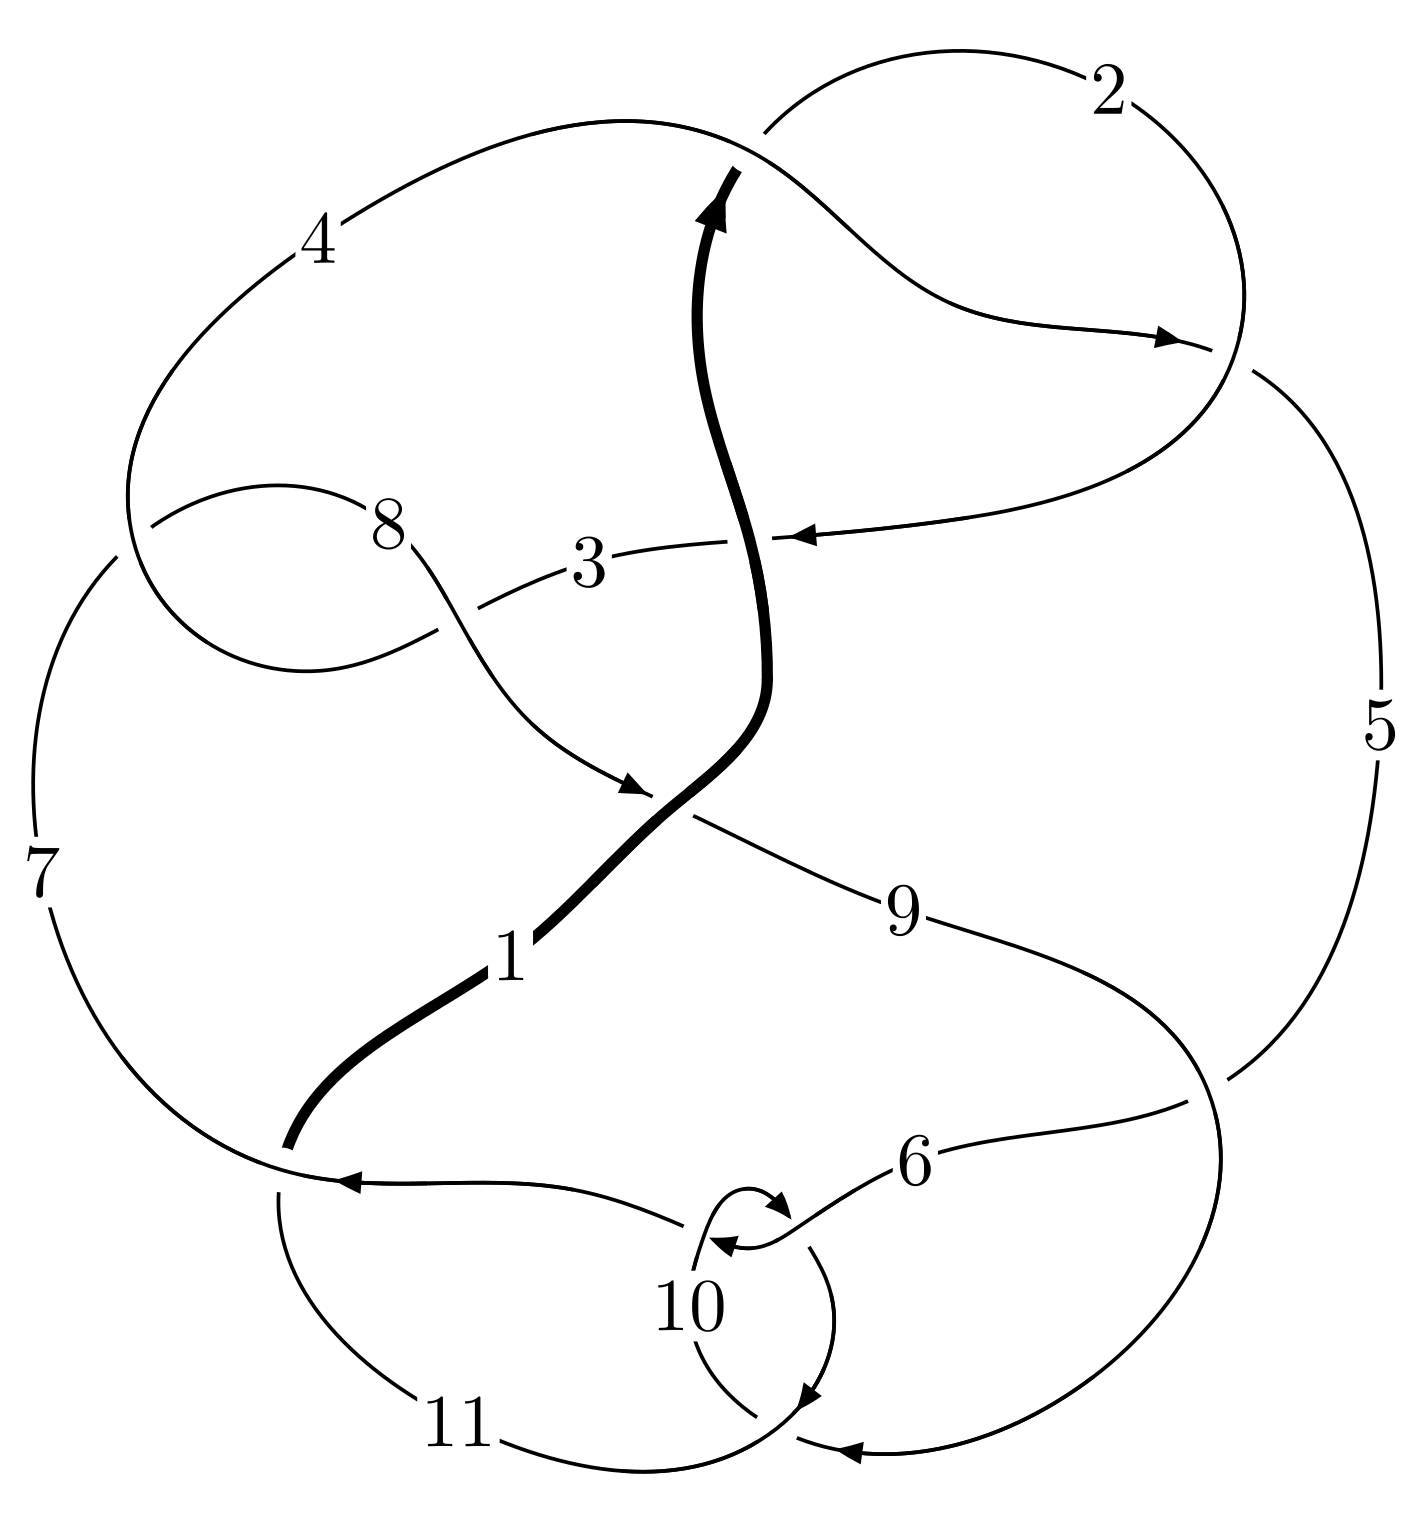
\includegraphics[width=112pt]{../../../GIT/diagram.site/Diagrams/png/669_11n_53.png}\\
\ \ \ A knot diagram\footnotemark}&
\allowdisplaybreaks
\textbf{Linearized knot diagam} \\
\cline{2-2}
 &
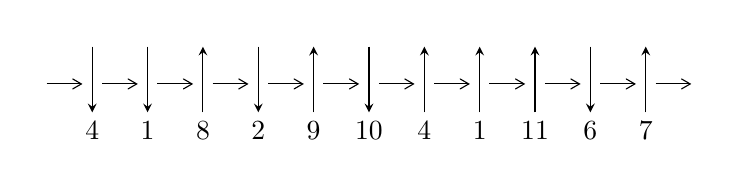
\begin{tikzpicture}[x=20pt, y=17pt]
	% nodes
	\node (C0) at (0, 0) {};
	\node (C1) at (1, 0) {};
	\node (C1U) at (1, +1) {};
	\node (C1D) at (1, -1) {4};

	\node (C2) at (2, 0) {};
	\node (C2U) at (2, +1) {};
	\node (C2D) at (2, -1) {1};

	\node (C3) at (3, 0) {};
	\node (C3U) at (3, +1) {};
	\node (C3D) at (3, -1) {8};

	\node (C4) at (4, 0) {};
	\node (C4U) at (4, +1) {};
	\node (C4D) at (4, -1) {2};

	\node (C5) at (5, 0) {};
	\node (C5U) at (5, +1) {};
	\node (C5D) at (5, -1) {9};

	\node (C6) at (6, 0) {};
	\node (C6U) at (6, +1) {};
	\node (C6D) at (6, -1) {10};

	\node (C7) at (7, 0) {};
	\node (C7U) at (7, +1) {};
	\node (C7D) at (7, -1) {4};

	\node (C8) at (8, 0) {};
	\node (C8U) at (8, +1) {};
	\node (C8D) at (8, -1) {1};

	\node (C9) at (9, 0) {};
	\node (C9U) at (9, +1) {};
	\node (C9D) at (9, -1) {11};

	\node (C10) at (10, 0) {};
	\node (C10U) at (10, +1) {};
	\node (C10D) at (10, -1) {6};

	\node (C11) at (11, 0) {};
	\node (C11U) at (11, +1) {};
	\node (C11D) at (11, -1) {7};
	\node (C12) at (12, 0) {};

	% arrows
	\draw[->,>={angle 60}]
	(C0) edge (C1) (C1) edge (C2) (C2) edge (C3) (C3) edge (C4) (C4) edge (C5) (C5) edge (C6) (C6) edge (C7) (C7) edge (C8) (C8) edge (C9) (C9) edge (C10) (C10) edge (C11) (C11) edge (C12) ;	\draw[->,>=stealth]
	(C1U) edge (C1D) (C2U) edge (C2D) (C3D) edge (C3U) (C4U) edge (C4D) (C5D) edge (C5U) (C6U) edge (C6D) (C7D) edge (C7U) (C8D) edge (C8U) (C9D) edge (C9U) (C10U) edge (C10D) (C11D) edge (C11U) ;
	\end{tikzpicture} \\
\hhline{~~} \\& 
\textbf{Solving Sequence} \\ \cline{2-2} 
 &
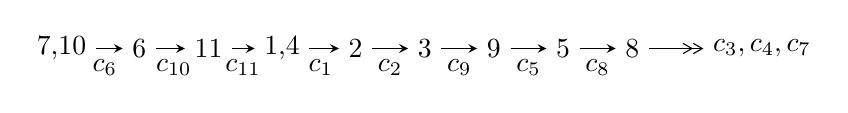
\begin{tikzpicture}[x=25pt, y=7pt]
	% node
	\node (A0) at (-1/8, 0) {7,10};
	\node (A1) at (1, 0) {6};
	\node (A2) at (2, 0) {11};
	\node (A3) at (49/16, 0) {1,4};
	\node (A4) at (33/8, 0) {2};
	\node (A5) at (41/8, 0) {3};
	\node (A6) at (49/8, 0) {9};
	\node (A7) at (57/8, 0) {5};
	\node (A8) at (65/8, 0) {8};
	\node (C1) at (1/2, -1) {$c_{6}$};
	\node (C2) at (3/2, -1) {$c_{10}$};
	\node (C3) at (5/2, -1) {$c_{11}$};
	\node (C4) at (29/8, -1) {$c_{1}$};
	\node (C5) at (37/8, -1) {$c_{2}$};
	\node (C6) at (45/8, -1) {$c_{9}$};
	\node (C7) at (53/8, -1) {$c_{5}$};
	\node (C8) at (61/8, -1) {$c_{8}$};
	\node (A9) at (10, 0) {$c_{3},c_{4},c_{7}$};

	% edge
	\draw[->,>=stealth]	
	(A0) edge (A1) (A1) edge (A2) (A2) edge (A3) (A3) edge (A4) (A4) edge (A5) (A5) edge (A6) (A6) edge (A7) (A7) edge (A8) ;
	\draw[->>,>={angle 60}]	
	(A8) edge (A9);
\end{tikzpicture} \\ 

\end{tabular} \\

\footnotetext{
The image of knot diagram is generated by the software ``\textbf{Draw programme}" developed by Andrew Bartholomew(\url{http://www.layer8.co.uk/maths/draw/index.htm\#Running-draw}), where we modified some parts for our purpose(\url{https://github.com/CATsTAILs/LinksPainter}).
}\phantom \\ \newline 
\centering \textbf{Ideals for irreducible components\footnotemark of $X_{\text{par}}$} 
 
\begin{align*}
I^u_{1}&=\langle 
- u^{22}+2 u^{21}+\cdots+b+1,\;u^{21}- u^{20}+\cdots+2 u^3+a,\;u^{23}-2 u^{22}+\cdots-2 u+1\rangle \\
I^u_{2}&=\langle 
b,\;- u^2+a- u-1,\;u^5+u^4+2 u^3+u^2+u+1\rangle \\
\\
\end{align*}
\raggedright * 2 irreducible components of $\dim_{\mathbb{C}}=0$, with total 28 representations.\\
\footnotetext{All coefficients of polynomials are rational numbers. But the coefficients are sometimes approximated in decimal forms when there is not enough margin.}
\newpage
\renewcommand{\arraystretch}{1}
\centering \section*{I. $I^u_{1}= \langle - u^{22}+2 u^{21}+\cdots+b+1,\;u^{21}- u^{20}+\cdots+2 u^3+a,\;u^{23}-2 u^{22}+\cdots-2 u+1 \rangle$}
\flushleft \textbf{(i) Arc colorings}\\
\begin{tabular}{m{7pt} m{180pt} m{7pt} m{180pt} }
\flushright $a_{7}=$&$\begin{pmatrix}1\\0\end{pmatrix}$ \\
\flushright $a_{10}=$&$\begin{pmatrix}0\\u\end{pmatrix}$ \\
\flushright $a_{6}=$&$\begin{pmatrix}1\\- u^2\end{pmatrix}$ \\
\flushright $a_{11}=$&$\begin{pmatrix}- u\\u^3+u\end{pmatrix}$ \\
\flushright $a_{1}=$&$\begin{pmatrix}u^3\\u^3+u\end{pmatrix}$ \\
\flushright $a_{4}=$&$\begin{pmatrix}- u^{21}+u^{20}+\cdots- u^4-2 u^3\\u^{22}-2 u^{21}+\cdots+2 u-1\end{pmatrix}$ \\
\flushright $a_{2}=$&$\begin{pmatrix}u^{18}- u^{17}+\cdots- u^2+u\\- u^8-2 u^6-2 u^4\end{pmatrix}$ \\
\flushright $a_{3}=$&$\begin{pmatrix}- u^{21}+u^{20}+\cdots+2 u-1\\u^{22}-2 u^{21}+\cdots+u-1\end{pmatrix}$ \\
\flushright $a_{9}=$&$\begin{pmatrix}- u^3\\u^5+u^3+u\end{pmatrix}$ \\
\flushright $a_{5}=$&$\begin{pmatrix}- u^6- u^4+1\\u^8+2 u^6+2 u^4\end{pmatrix}$ \\
\flushright $a_{8}=$&$\begin{pmatrix}- u^{11}-2 u^9-2 u^7- u^3\\- u^{11}-3 u^9-4 u^7- u^5+u^3+u\end{pmatrix}$\\ \flushright $a_{8}=$&$\begin{pmatrix}- u^{11}-2 u^9-2 u^7- u^3\\- u^{11}-3 u^9-4 u^7- u^5+u^3+u\end{pmatrix}$\\&\end{tabular}
\flushleft \textbf{(ii) Obstruction class $= -1$}\\~\\
\flushleft \textbf{(iii) Cusp Shapes $= 4 u^{22}-9 u^{21}+30 u^{20}-48 u^{19}+96 u^{18}-131 u^{17}+190 u^{16}-224 u^{15}+249 u^{14}-262 u^{13}+237 u^{12}-210 u^{11}+148 u^{10}-93 u^9+53 u^8-6 u^7-14 u^6+25 u^5-18 u^4-10 u^2+9 u-5$}\\~\\
\newpage\renewcommand{\arraystretch}{1}
\flushleft \textbf{(iv) u-Polynomials at the component}\newline \\
\begin{tabular}{m{50pt}|m{274pt}}
Crossings & \hspace{64pt}u-Polynomials at each crossing \\
\hline $$\begin{aligned}c_{1},c_{4}\end{aligned}$$&$\begin{aligned}
&u^{23}-6 u^{22}+\cdots+4 u-1
\end{aligned}$\\
\hline $$\begin{aligned}c_{2}\end{aligned}$$&$\begin{aligned}
&u^{23}+32 u^{22}+\cdots-16 u+1
\end{aligned}$\\
\hline $$\begin{aligned}c_{3},c_{7}\end{aligned}$$&$\begin{aligned}
&u^{23}- u^{22}+\cdots+32 u-32
\end{aligned}$\\
\hline $$\begin{aligned}c_{5},c_{11}\end{aligned}$$&$\begin{aligned}
&u^{23}-2 u^{22}+\cdots+30 u-9
\end{aligned}$\\
\hline $$\begin{aligned}c_{6},c_{10}\end{aligned}$$&$\begin{aligned}
&u^{23}+2 u^{22}+\cdots-2 u-1
\end{aligned}$\\
\hline $$\begin{aligned}c_{8}\end{aligned}$$&$\begin{aligned}
&u^{23}+24 u^{21}+\cdots+2 u-1
\end{aligned}$\\
\hline $$\begin{aligned}c_{9}\end{aligned}$$&$\begin{aligned}
&u^{23}-12 u^{22}+\cdots-2 u+1
\end{aligned}$\\
\hline
\end{tabular}\\~\\
\newpage\renewcommand{\arraystretch}{1}
\flushleft \textbf{(v) Riley Polynomials at the component}\newline \\
\begin{tabular}{m{50pt}|m{274pt}}
Crossings & \hspace{64pt}Riley Polynomials at each crossing \\
\hline $$\begin{aligned}c_{1},c_{4}\end{aligned}$$&$\begin{aligned}
&y^{23}-32 y^{22}+\cdots-16 y-1
\end{aligned}$\\
\hline $$\begin{aligned}c_{2}\end{aligned}$$&$\begin{aligned}
&y^{23}-76 y^{22}+\cdots+772 y-1
\end{aligned}$\\
\hline $$\begin{aligned}c_{3},c_{7}\end{aligned}$$&$\begin{aligned}
&y^{23}+33 y^{22}+\cdots+3584 y-1024
\end{aligned}$\\
\hline $$\begin{aligned}c_{5},c_{11}\end{aligned}$$&$\begin{aligned}
&y^{23}-12 y^{22}+\cdots-162 y-81
\end{aligned}$\\
\hline $$\begin{aligned}c_{6},c_{10}\end{aligned}$$&$\begin{aligned}
&y^{23}+12 y^{22}+\cdots-2 y-1
\end{aligned}$\\
\hline $$\begin{aligned}c_{8}\end{aligned}$$&$\begin{aligned}
&y^{23}+48 y^{22}+\cdots-2 y-1
\end{aligned}$\\
\hline $$\begin{aligned}c_{9}\end{aligned}$$&$\begin{aligned}
&y^{23}+24 y^{21}+\cdots-6 y-1
\end{aligned}$\\
\hline
\end{tabular}\\~\\
\newpage\flushleft \textbf{(vi) Complex Volumes and Cusp Shapes}
$$\begin{array}{c|c|c}  
\text{Solutions to }I^u_{1}& \I (\text{vol} + \sqrt{-1}CS) & \text{Cusp shape}\\
 \hline 
\begin{aligned}
u &= -0.700458 + 0.794163 I \\
a &= -1.45877 + 0.07887 I \\
b &= -0.09416 - 2.13003 I\end{aligned}
 & -14.1192 + 2.6463 I & -3.65714 - 2.84707 I \\ \hline\begin{aligned}
u &= -0.700458 - 0.794163 I \\
a &= -1.45877 - 0.07887 I \\
b &= -0.09416 + 2.13003 I\end{aligned}
 & -14.1192 - 2.6463 I & -3.65714 + 2.84707 I \\ \hline\begin{aligned}
u &= \phantom{-}0.855800 + 0.265895 I \\
a &= -0.795468 - 0.188526 I \\
b &= -0.45428 - 1.93201 I\end{aligned}
 & -11.07970 + 5.13429 I & -2.96602 - 2.08249 I \\ \hline\begin{aligned}
u &= \phantom{-}0.855800 - 0.265895 I \\
a &= -0.795468 + 0.188526 I \\
b &= -0.45428 + 1.93201 I\end{aligned}
 & -11.07970 - 5.13429 I & -2.96602 + 2.08249 I \\ \hline\begin{aligned}
u &= \phantom{-}0.366516 + 1.072630 I \\
a &= \phantom{-}0.312367 - 0.791611 I \\
b &= -0.215406 - 0.997383 I\end{aligned}
 & \phantom{-}1.62847 - 1.16584 I & \phantom{-}3.47504 + 0.42481 I \\ \hline\begin{aligned}
u &= \phantom{-}0.366516 - 1.072630 I \\
a &= \phantom{-}0.312367 + 0.791611 I \\
b &= -0.215406 + 0.997383 I\end{aligned}
 & \phantom{-}1.62847 + 1.16584 I & \phantom{-}3.47504 - 0.42481 I \\ \hline\begin{aligned}
u &= -0.477094 + 1.041350 I \\
a &= \phantom{-}2.43046 - 1.25941 I \\
b &= \phantom{-}1.105500 + 0.395247 I\end{aligned}
 & -0.82985 + 3.19017 I & \phantom{-}0.92409 - 4.72756 I \\ \hline\begin{aligned}
u &= -0.477094 - 1.041350 I \\
a &= \phantom{-}2.43046 + 1.25941 I \\
b &= \phantom{-}1.105500 - 0.395247 I\end{aligned}
 & -0.82985 - 3.19017 I & \phantom{-}0.92409 + 4.72756 I \\ \hline\begin{aligned}
u &= \phantom{-}0.270789 + 0.755843 I \\
a &= \phantom{-}0.693663 + 0.260910 I \\
b &= \phantom{-}0.349805 - 0.349927 I\end{aligned}
 & \phantom{-}0.390924 - 1.217980 I & \phantom{-}4.26810 + 5.45735 I \\ \hline\begin{aligned}
u &= \phantom{-}0.270789 - 0.755843 I \\
a &= \phantom{-}0.693663 - 0.260910 I \\
b &= \phantom{-}0.349805 + 0.349927 I\end{aligned}
 & \phantom{-}0.390924 + 1.217980 I & \phantom{-}4.26810 - 5.45735 I\\
 \hline 
 \end{array}$$\newpage$$\begin{array}{c|c|c}  
\text{Solutions to }I^u_{1}& \I (\text{vol} + \sqrt{-1}CS) & \text{Cusp shape}\\
 \hline 
\begin{aligned}
u &= \phantom{-}0.514060 + 1.104640 I \\
a &= -1.31154 + 0.63853 I \\
b &= \phantom{-}0.143374 + 1.329070 I\end{aligned}
 & \phantom{-}0.55803 - 6.09572 I & \phantom{-}0.93537 + 6.19372 I \\ \hline\begin{aligned}
u &= \phantom{-}0.514060 - 1.104640 I \\
a &= -1.31154 - 0.63853 I \\
b &= \phantom{-}0.143374 - 1.329070 I\end{aligned}
 & \phantom{-}0.55803 + 6.09572 I & \phantom{-}0.93537 - 6.19372 I \\ \hline\begin{aligned}
u &= -0.455035 + 1.182370 I \\
a &= -1.061190 + 0.524858 I \\
b &= -0.608111 - 0.025252 I\end{aligned}
 & \phantom{-}5.15559 + 4.27437 I & \phantom{-}9.78577 - 3.28837 I \\ \hline\begin{aligned}
u &= -0.455035 - 1.182370 I \\
a &= -1.061190 - 0.524858 I \\
b &= -0.608111 + 0.025252 I\end{aligned}
 & \phantom{-}5.15559 - 4.27437 I & \phantom{-}9.78577 + 3.28837 I \\ \hline\begin{aligned}
u &= \phantom{-}0.269522 + 1.238660 I \\
a &= \phantom{-}0.24803 + 2.58133 I \\
b &= \phantom{-}0.34057 + 1.76704 I\end{aligned}
 & -6.23110 + 1.56382 I & \phantom{-}1.72734 - 0.04821 I \\ \hline\begin{aligned}
u &= \phantom{-}0.269522 - 1.238660 I \\
a &= \phantom{-}0.24803 - 2.58133 I \\
b &= \phantom{-}0.34057 - 1.76704 I\end{aligned}
 & -6.23110 - 1.56382 I & \phantom{-}1.72734 + 0.04821 I \\ \hline\begin{aligned}
u &= -0.719779\phantom{ +0.000000I} \\
a &= \phantom{-}0.526584\phantom{ +0.000000I} \\
b &= \phantom{-}0.562756\phantom{ +0.000000I}\end{aligned}
 & \phantom{-}1.81820\phantom{ +0.000000I} & \phantom{-}6.35980\phantom{ +0.000000I} \\ \hline\begin{aligned}
u &= \phantom{-}0.573488 + 1.178530 I \\
a &= \phantom{-}2.84278 - 1.00616 I \\
b &= \phantom{-}0.57374 - 1.89861 I\end{aligned}
 & -8.35091 - 10.39480 I & -0.03516 + 5.66347 I \\ \hline\begin{aligned}
u &= \phantom{-}0.573488 - 1.178530 I \\
a &= \phantom{-}2.84278 + 1.00616 I \\
b &= \phantom{-}0.57374 + 1.89861 I\end{aligned}
 & -8.35091 + 10.39480 I & -0.03516 - 5.66347 I \\ \hline\begin{aligned}
u &= -0.469209 + 0.502755 I \\
a &= -0.699918 - 0.973698 I \\
b &= -0.674614 + 0.656598 I\end{aligned}
 & -2.46377 + 0.78545 I & -4.30142 - 0.09221 I\\
 \hline 
 \end{array}$$\newpage$$\begin{array}{c|c|c}  
\text{Solutions to }I^u_{1}& \I (\text{vol} + \sqrt{-1}CS) & \text{Cusp shape}\\
 \hline 
\begin{aligned}
u &= -0.469209 - 0.502755 I \\
a &= -0.699918 + 0.973698 I \\
b &= -0.674614 - 0.656598 I\end{aligned}
 & -2.46377 - 0.78545 I & -4.30142 + 0.09221 I \\ \hline\begin{aligned}
u &= \phantom{-}0.611511 + 0.287188 I \\
a &= \phantom{-}0.036277 - 0.858010 I \\
b &= -0.247796 + 1.071450 I\end{aligned}
 & -1.75612 + 1.64275 I & -3.33585 - 2.40342 I \\ \hline\begin{aligned}
u &= \phantom{-}0.611511 - 0.287188 I \\
a &= \phantom{-}0.036277 + 0.858010 I \\
b &= -0.247796 - 1.071450 I\end{aligned}
 & -1.75612 - 1.64275 I & -3.33585 + 2.40342 I\\
 \hline 
 \end{array}$$\newpage\newpage\renewcommand{\arraystretch}{1}
\centering \section*{II. $I^u_{2}= \langle b,\;- u^2+a- u-1,\;u^5+u^4+2 u^3+u^2+u+1 \rangle$}
\flushleft \textbf{(i) Arc colorings}\\
\begin{tabular}{m{7pt} m{180pt} m{7pt} m{180pt} }
\flushright $a_{7}=$&$\begin{pmatrix}1\\0\end{pmatrix}$ \\
\flushright $a_{10}=$&$\begin{pmatrix}0\\u\end{pmatrix}$ \\
\flushright $a_{6}=$&$\begin{pmatrix}1\\- u^2\end{pmatrix}$ \\
\flushright $a_{11}=$&$\begin{pmatrix}- u\\u^3+u\end{pmatrix}$ \\
\flushright $a_{1}=$&$\begin{pmatrix}u^3\\u^3+u\end{pmatrix}$ \\
\flushright $a_{4}=$&$\begin{pmatrix}u^2+u+1\\0\end{pmatrix}$ \\
\flushright $a_{2}=$&$\begin{pmatrix}u^3+u^2+u+1\\u^3+u\end{pmatrix}$ \\
\flushright $a_{3}=$&$\begin{pmatrix}u^2+u+1\\0\end{pmatrix}$ \\
\flushright $a_{9}=$&$\begin{pmatrix}- u^3\\- u^4- u^3- u^2-1\end{pmatrix}$ \\
\flushright $a_{5}=$&$\begin{pmatrix}- u^3\\- u^3- u\end{pmatrix}$ \\
\flushright $a_{8}=$&$\begin{pmatrix}1\\0\end{pmatrix}$\\ \flushright $a_{8}=$&$\begin{pmatrix}1\\0\end{pmatrix}$\\&\end{tabular}
\flushleft \textbf{(ii) Obstruction class $= 1$}\\~\\
\flushleft \textbf{(iii) Cusp Shapes $= -2 u^4+u^3+2 u$}\\~\\
\newpage\renewcommand{\arraystretch}{1}
\flushleft \textbf{(iv) u-Polynomials at the component}\newline \\
\begin{tabular}{m{50pt}|m{274pt}}
Crossings & \hspace{64pt}u-Polynomials at each crossing \\
\hline $$\begin{aligned}c_{1}\end{aligned}$$&$\begin{aligned}
&(u-1)^5
\end{aligned}$\\
\hline $$\begin{aligned}c_{2},c_{4}\end{aligned}$$&$\begin{aligned}
&(u+1)^5
\end{aligned}$\\
\hline $$\begin{aligned}c_{3},c_{7}\end{aligned}$$&$\begin{aligned}
&u^5
\end{aligned}$\\
\hline $$\begin{aligned}c_{5},c_{8}\end{aligned}$$&$\begin{aligned}
&u^5- u^4-2 u^3+u^2+u+1
\end{aligned}$\\
\hline $$\begin{aligned}c_{6}\end{aligned}$$&$\begin{aligned}
&u^5+u^4+2 u^3+u^2+u+1
\end{aligned}$\\
\hline $$\begin{aligned}c_{9}\end{aligned}$$&$\begin{aligned}
&u^5+3 u^4+4 u^3+u^2- u-1
\end{aligned}$\\
\hline $$\begin{aligned}c_{10}\end{aligned}$$&$\begin{aligned}
&u^5- u^4+2 u^3- u^2+u-1
\end{aligned}$\\
\hline $$\begin{aligned}c_{11}\end{aligned}$$&$\begin{aligned}
&u^5+u^4-2 u^3- u^2+u-1
\end{aligned}$\\
\hline
\end{tabular}\\~\\
\newpage\renewcommand{\arraystretch}{1}
\flushleft \textbf{(v) Riley Polynomials at the component}\newline \\
\begin{tabular}{m{50pt}|m{274pt}}
Crossings & \hspace{64pt}Riley Polynomials at each crossing \\
\hline $$\begin{aligned}c_{1},c_{2},c_{4}\end{aligned}$$&$\begin{aligned}
&(y-1)^5
\end{aligned}$\\
\hline $$\begin{aligned}c_{3},c_{7}\end{aligned}$$&$\begin{aligned}
&y^5
\end{aligned}$\\
\hline $$\begin{aligned}c_{5},c_{8},c_{11}\end{aligned}$$&$\begin{aligned}
&y^5-5 y^4+8 y^3-3 y^2- y-1
\end{aligned}$\\
\hline $$\begin{aligned}c_{6},c_{10}\end{aligned}$$&$\begin{aligned}
&y^5+3 y^4+4 y^3+y^2- y-1
\end{aligned}$\\
\hline $$\begin{aligned}c_{9}\end{aligned}$$&$\begin{aligned}
&y^5- y^4+8 y^3-3 y^2+3 y-1
\end{aligned}$\\
\hline
\end{tabular}\\~\\
\newpage\flushleft \textbf{(vi) Complex Volumes and Cusp Shapes}
$$\begin{array}{c|c|c}  
\text{Solutions to }I^u_{2}& \I (\text{vol} + \sqrt{-1}CS) & \text{Cusp shape}\\
 \hline 
\begin{aligned}
u &= \phantom{-}0.339110 + 0.822375 I \\
a &= \phantom{-}0.77780 + 1.38013 I \\
b &= \phantom{-0.000000 } 0\end{aligned}
 & -1.31583 - 1.53058 I & \phantom{-}0.02124 + 2.62456 I \\ \hline\begin{aligned}
u &= \phantom{-}0.339110 - 0.822375 I \\
a &= \phantom{-}0.77780 - 1.38013 I \\
b &= \phantom{-0.000000 } 0\end{aligned}
 & -1.31583 + 1.53058 I & \phantom{-}0.02124 - 2.62456 I \\ \hline\begin{aligned}
u &= -0.766826\phantom{ +0.000000I} \\
a &= \phantom{-}0.821196\phantom{ +0.000000I} \\
b &= \phantom{-0.000000 } 0\end{aligned}
 & \phantom{-}0.756147\phantom{ +0.000000I} & -2.67610\phantom{ +0.000000I} \\ \hline\begin{aligned}
u &= -0.455697 + 1.200150 I \\
a &= -0.688402 + 0.106340 I \\
b &= \phantom{-0.000000 } 0\end{aligned}
 & \phantom{-}4.22763 + 4.40083 I & \phantom{-}0.31681 - 3.97407 I \\ \hline\begin{aligned}
u &= -0.455697 - 1.200150 I \\
a &= -0.688402 - 0.106340 I \\
b &= \phantom{-0.000000 } 0\end{aligned}
 & \phantom{-}4.22763 - 4.40083 I & \phantom{-}0.31681 + 3.97407 I\\
 \hline 
 \end{array}$$\newpage
\newpage\renewcommand{\arraystretch}{1}
\centering \section*{ III. u-Polynomials}
\begin{tabular}{m{50pt}|m{274pt}}
Crossings & \hspace{64pt}u-Polynomials at each crossing \\
\hline $$\begin{aligned}c_{1}\end{aligned}$$&$\begin{aligned}
&((u-1)^5)(u^{23}-6 u^{22}+\cdots+4 u-1)
\end{aligned}$\\
\hline $$\begin{aligned}c_{2}\end{aligned}$$&$\begin{aligned}
&((u+1)^5)(u^{23}+32 u^{22}+\cdots-16 u+1)
\end{aligned}$\\
\hline $$\begin{aligned}c_{3},c_{7}\end{aligned}$$&$\begin{aligned}
&u^5(u^{23}- u^{22}+\cdots+32 u-32)
\end{aligned}$\\
\hline $$\begin{aligned}c_{4}\end{aligned}$$&$\begin{aligned}
&((u+1)^5)(u^{23}-6 u^{22}+\cdots+4 u-1)
\end{aligned}$\\
\hline $$\begin{aligned}c_{5}\end{aligned}$$&$\begin{aligned}
&(u^5- u^4-2 u^3+u^2+u+1)(u^{23}-2 u^{22}+\cdots+30 u-9)
\end{aligned}$\\
\hline $$\begin{aligned}c_{6}\end{aligned}$$&$\begin{aligned}
&(u^5+u^4+2 u^3+u^2+u+1)(u^{23}+2 u^{22}+\cdots-2 u-1)
\end{aligned}$\\
\hline $$\begin{aligned}c_{8}\end{aligned}$$&$\begin{aligned}
&(u^5- u^4-2 u^3+u^2+u+1)(u^{23}+24 u^{21}+\cdots+2 u-1)
\end{aligned}$\\
\hline $$\begin{aligned}c_{9}\end{aligned}$$&$\begin{aligned}
&(u^5+3 u^4+4 u^3+u^2- u-1)(u^{23}-12 u^{22}+\cdots-2 u+1)
\end{aligned}$\\
\hline $$\begin{aligned}c_{10}\end{aligned}$$&$\begin{aligned}
&(u^5- u^4+2 u^3- u^2+u-1)(u^{23}+2 u^{22}+\cdots-2 u-1)
\end{aligned}$\\
\hline $$\begin{aligned}c_{11}\end{aligned}$$&$\begin{aligned}
&(u^5+u^4-2 u^3- u^2+u-1)(u^{23}-2 u^{22}+\cdots+30 u-9)
\end{aligned}$\\
\hline
\end{tabular}\newpage\renewcommand{\arraystretch}{1}
\centering \section*{ IV. Riley Polynomials}
\begin{tabular}{m{50pt}|m{274pt}}
Crossings & \hspace{64pt}Riley Polynomials at each crossing \\
\hline $$\begin{aligned}c_{1},c_{4}\end{aligned}$$&$\begin{aligned}
&((y-1)^5)(y^{23}-32 y^{22}+\cdots-16 y-1)
\end{aligned}$\\
\hline $$\begin{aligned}c_{2}\end{aligned}$$&$\begin{aligned}
&((y-1)^5)(y^{23}-76 y^{22}+\cdots+772 y-1)
\end{aligned}$\\
\hline $$\begin{aligned}c_{3},c_{7}\end{aligned}$$&$\begin{aligned}
&y^5(y^{23}+33 y^{22}+\cdots+3584 y-1024)
\end{aligned}$\\
\hline $$\begin{aligned}c_{5},c_{11}\end{aligned}$$&$\begin{aligned}
&(y^5-5 y^4+8 y^3-3 y^2- y-1)(y^{23}-12 y^{22}+\cdots-162 y-81)
\end{aligned}$\\
\hline $$\begin{aligned}c_{6},c_{10}\end{aligned}$$&$\begin{aligned}
&(y^5+3 y^4+4 y^3+y^2- y-1)(y^{23}+12 y^{22}+\cdots-2 y-1)
\end{aligned}$\\
\hline $$\begin{aligned}c_{8}\end{aligned}$$&$\begin{aligned}
&(y^5-5 y^4+8 y^3-3 y^2- y-1)(y^{23}+48 y^{22}+\cdots-2 y-1)
\end{aligned}$\\
\hline $$\begin{aligned}c_{9}\end{aligned}$$&$\begin{aligned}
&(y^5- y^4+8 y^3-3 y^2+3 y-1)(y^{23}+24 y^{21}+\cdots-6 y-1)
\end{aligned}$\\
\hline
\end{tabular}
\vskip 2pc
\end{document}